\chapter{تطبيقات الترموديناميك الإحصائي}\label{ch:b3:statistical-thermo-applied}

الهيدروجين السائل المحفوظ في أفضل الخزانات عزلًا يتبخر مع ذلك، وفي
الأيام الأولى بعد تسييله يتبخر أسرع بكثير مما تفسره الحرارة المتسربة
عبر الجدران. فالحرارة تأتي من داخل السائل. فجزيئات الهيدروجين
توجد في صورتين، لا تختلفان إلا في الاتجاه النسبي
لسبيني بروتونيهما، ولا تتحول إحداهما إلى الأخرى إلا ببطء
شديد؛ وعند \qty{20}{K} يحرر تحول إحدى الصورتين إلى الأخرى حرارة
تفوق ما يلزم لتبخير السائل. يطبّق هذا الفصل
دوال التجزئة في \cref{ch:b3:partition-functions} على السعات الحرارية، وعلى
هذين المتماكبين السبينيين النوويين وعلى الإنتروبيا التي تحتفظ بها بعض البلورات عند 0 K،
ثم يحسب ثوابت التوازن والمفاعيل النظائرية من المعطيات الطيفية
وحدها.

\begin{recall}
بنى \cref{ch:b3:partition-functions} \omterm{def:b3:partition-functions:partition-function}{دالة التجزئة الجزيئية} 
وعواملها الأربعة، واستنتج منها $U$ و$S$ و$G$. وربط مجلد السنة الثانية
ثابت التوازن القياسي بطاقة جيبس القياسية للتفاعل،
$\Delta_rG^\circ = -RT\ln K^\circ$، وأثبت معادلة فانت هوف؛
وذكر \cref{ch:b3:many-electron-atoms} أن الدالة الموجية تغيّر إشارتها حين يتبادل
فرميونان متطابقان؛ ووجد \cref{ch:b3:rovibrational-spectroscopy}
تناوب شدات الخطوط بنسبة 3:1 في طيف رامان الدوراني لجزيئات شبيهة
بالجزيء \ce{H2}. وعرّف جزء الصف التاسع من المجلد الأول النظائر.
\end{recall}

\begin{omfigure}
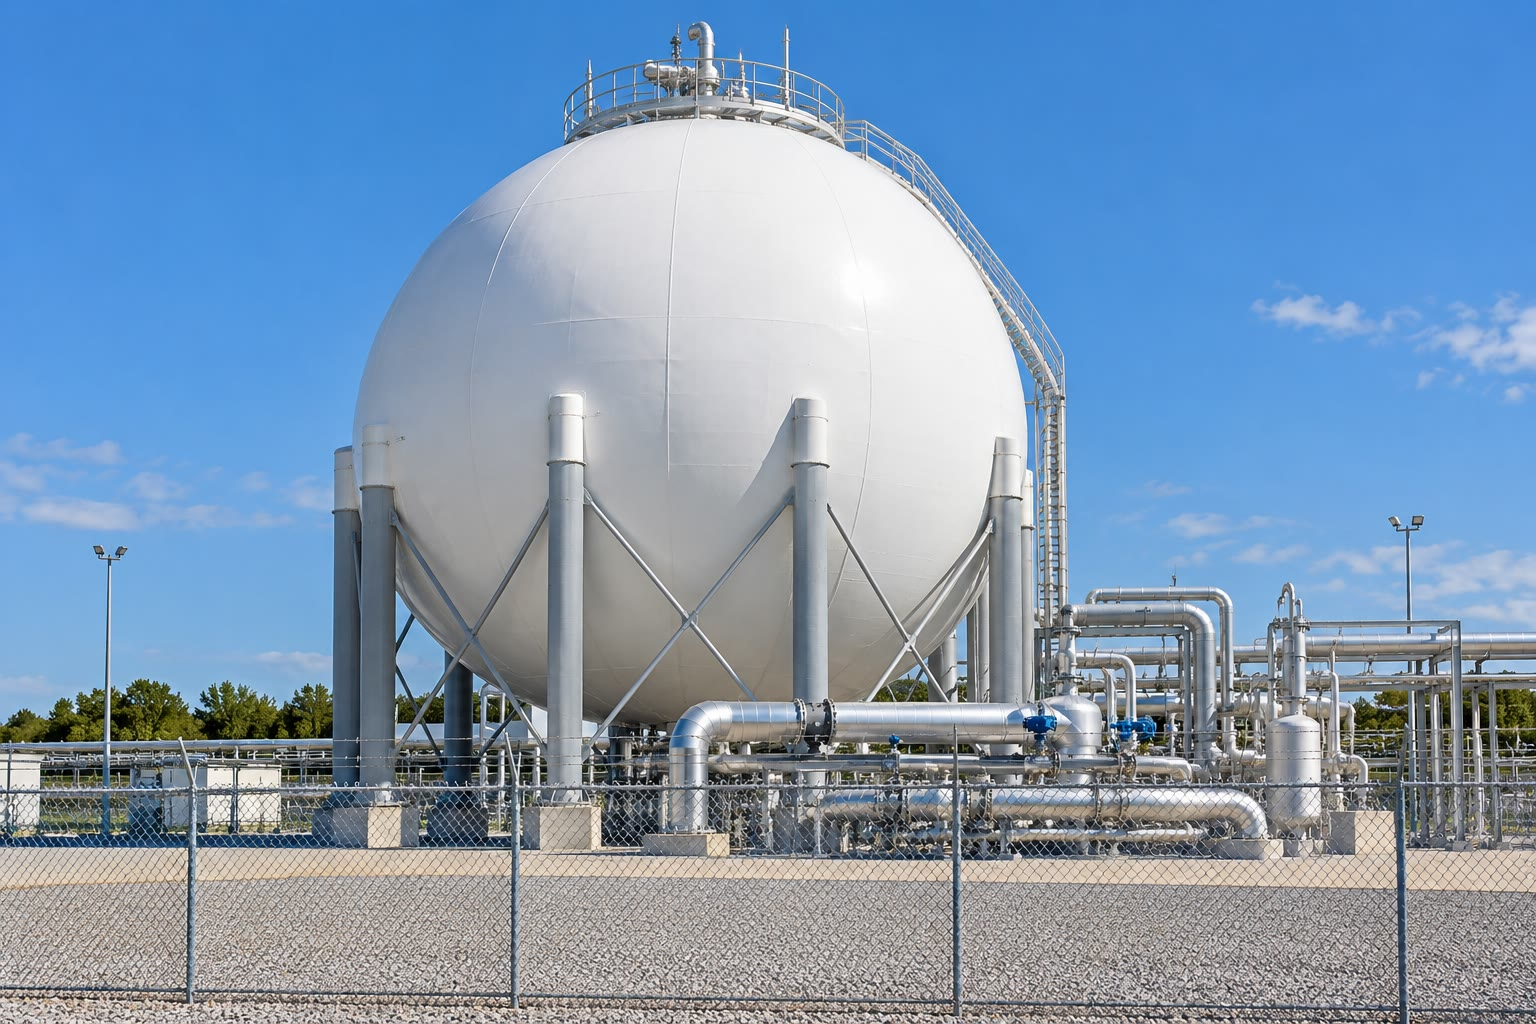
\includegraphics[width=0.6\linewidth]{images/book4/ai/b3-11-lh2-tank.jpg}

{\small خزان كروي للهيدروجين السائل. عند \qty{20}{K}، قد تتجاوز الحرارة المتولدة داخل
السائل بفعل التحول البطيء لإحدى الصورتين السبينيتين النوويتين للهيدروجين إلى
الأخرى الحرارةَ المتسربة من الخارج.}
\end{omfigure}

\section{السعات الحرارية للغازات}

السعة الحرارية عند حجم ثابت هي $C_V = (\partial U/\partial T)_V$، ومع
\cref{thm:b3:partition-functions:internal-energy} يساهم كل نوع من الحركة
على حدة. ونهايتان تحكمان كل شيء.

\begin{theorem}[مبرهنة التوزيع المتساوي]\label{thm:b3:statistical-thermo-applied:equipartition}
حين تكون مستويات طاقة حركة ما متقاربة مقارنةً بالمقدار $kT$، فإن كل
حد من طاقتها تربيعي في إحداثي أو في كمية حركة يساهم بالمقدار
$\frac12kT$ في متوسط طاقة الجزيء، ومنه بالمقدار $\frac12R$ في السعة الحرارية
المولية. وهذا القول هو \emph{مبرهنة التوزيع المتساوي}\index{مبرهنة التوزيع المتساوي}.
\end{theorem}

\begin{proof}[برهان جزئي]
في النهاية الكلاسيكية يصير المجموع على حالات حركة ما
تكاملًا، ويساهم الحد التربيعي $a u^2$ بالعامل $\int\eu^{-\beta au^2}\dd u =
\sqrt{\pi/\beta a}$، المتناسب مع $\beta^{-1/2}$. وبحسب
\cref{thm:b3:partition-functions:internal-energy}، يكون متوسط طاقته
$-\partial\ln(\beta^{-1/2})/\partial\beta = 1/2\beta = \frac12kT$. أما أن التكامل الكلاسيكي هو
نهاية المجموع الكمومي فقد بُيّن للانسحاب والدوران في
\cref{ch:b3:partition-functions}؛ وهو ينتج للاهتزاز من القضية
التالية حين $T \gg \theta_{\mathrm V}$.
\end{proof}

للانسحاب ثلاثة حدود تربيعية ($\frac32R$)؛ ولدوران الجزيء الخطي
حدان ($R$)، وللجزيء غير الخطي ثلاثة ($\frac32R$)؛ ولكل اهتزاز حدان،
حركي وكامن ($R$). فالجزيء الخطي ذو $N$ ذرة يؤول إذن إلى
$C_{V,\mathrm m} = \frac52R + (3N - 5)R$ في درجة حرارة مرتفعة. ولا تكاد هذه النهاية
تُبلغ أبدًا للاهتزازات في درجة حرارة الغرفة.

\begin{proposition}[السعة الحرارية الاهتزازية]\label{prop:b3:statistical-thermo-applied:cv-vib}
يساهم اهتزاز توافقي درجة حرارته المميزة $\theta_{\mathrm V}$، مع
$x = \theta_{\mathrm V}/T$، بالمقدار
\[
  \frac{C_{V,\mathrm m}^{\mathrm V}}{R} = \frac{x^2\eu^x}{(\eu^x - 1)^2},
\]
وهي دالة أينشتاين، التي تؤول إلى 1 حين $T \gg \theta_{\mathrm V}$ وتتناقص
أسيًا، كالمقدار $x^2\eu^{-x}$، حين $T \ll \theta_{\mathrm V}$.
\end{proposition}

\begin{proof}
من \cref{prop:b3:partition-functions:q-vib}، $U - U(0) = R\theta_{\mathrm V}/(\eu^x - 1)$ لكل مول.
وبالاشتقاق بالنسبة إلى $T$، مع $\dd x/\dd T = -x/T$، نحصل على
$R\theta_{\mathrm V}\eu^x(x/T)/(\eu^x - 1)^2 = Rx^2\eu^x/(\eu^x - 1)^2$. ومن أجل $x \to 0$، $\eu^x - 1 \approx x$ 
وتؤول النسبة إلى 1؛ ومن أجل $x$ الكبيرة تسلك سلوك $x^2\eu^{-x}$.
\end{proof}

\begin{method}[السعة الحرارية لغاز من أنماطه]\label{met:b3:statistical-thermo-applied:cv}
\begin{enumerate}
  \item الانسحاب: $\frac32R$، دائمًا.
  \item الدوران: $R$ (خطي) أو $\frac32R$ (غير خطي) إذا كان $T \gg \theta_{\mathrm R}$، وهذا صحيح لكل
        غاز عدا الهيدروجين فوق بضع عشرات من الكلفنات.
  \item الاهتزازات: حد أينشتاين واحد لكل \omterm{def:b3:group-theory-applied:normal-mode}{نمط عادي}، مع $\theta_{\mathrm V} = hc\tilde\nu/k$ من
        الأعداد الموجية للانتقالات الأساسية؛ والنمط المنحل يُعدّ بقدر
        \omterm{def:b3:quantum-model-systems:degenerate}{درجة انحلاله}.
  \item اجمع، و$C_{p,\mathrm m} = C_{V,\mathrm m} + R$ لغاز مثالي.
\end{enumerate}
\end{method}

يُقال عن حركة إنها مجمّدة حين يكون $kT$ صغيرًا مقارنةً بأول
إثارة لها: فهي لا تحمل عندئذ أي طاقة ولا تساهم بشيء في $C_V$. 
واهتزاز \ce{N2} ($\theta_{\mathrm V} = \qty{3352}{K}$) مجمّد في درجة حرارة الغرفة 
و$C_{V,\mathrm m} = \frac52R$؛ أما اهتزاز \ce{Cl2} ($\theta_{\mathrm V} = \qty{798}{K}$) فنصف مستيقظ،
$C_{V,\mathrm m} = 3.07R$ عند \qty{300}{K}.

\begin{omfigure}
\begin{tikzpicture}
\begin{axis}[width=0.86\linewidth, height=6.4cm, xmode=log, xmin=10, xmax=3000,
  ymin=1.3, ymax=3.9, axis lines=left, xlabel={\babelsublr{$T$ / K}}, ylabel={$C_{V,\mathrm m}/R$},
  tick label style={font=\small}, label style={font=\small},
  log ticks with fixed point, xtick={10,30,100,300,1000,3000},
  unbounded coords=jump]
\addplot[omDef, thick] table[x=T, y=N2] {figdata/out/bachelor-3-heat-capacity.dat};
\addplot[black!60, thick] table[x=T, y=Cl2] {figdata/out/bachelor-3-heat-capacity.dat};
\addplot[omThm, thick, dashed] table[x=T, y=nH2] {figdata/out/bachelor-3-heat-capacity.dat};
\addplot[omThm, thick] table[x=T, y=eH2] {figdata/out/bachelor-3-heat-capacity.dat};
\addplot[only marks, mark=*, mark size=1.6pt, omDef] table[x=T, y=N2] {figdata/out/bachelor-3-heat-capacity-janaf.dat};
\addplot[only marks, mark=square*, mark size=1.5pt, black!60] table[x=T, y=Cl2] {figdata/out/bachelor-3-heat-capacity-janaf.dat};
\draw[black!30, densely dotted] (axis cs:10,1.5) -- (axis cs:3000,1.5);
\draw[black!30, densely dotted] (axis cs:10,2.5) -- (axis cs:3000,2.5);
\draw[black!30, densely dotted] (axis cs:10,3.5) -- (axis cs:3000,3.5);
\node[font=\scriptsize, black!60, anchor=south east] at (axis cs:2900,1.5) {\foreignlanguage{arabic}{$\frac32$: الانسحاب}};
\node[font=\scriptsize, black!60, anchor=south west] at (axis cs:10.5,2.5) {\foreignlanguage{arabic}{$\frac52$: + الدوران}};
\node[font=\scriptsize, black!60, anchor=south west] at (axis cs:10.5,3.5) {\foreignlanguage{arabic}{$\frac72$: + الاهتزاز}};
\node[font=\scriptsize, omThm, anchor=south west] at (axis cs:60,3.6) {\foreignlanguage{arabic}{\ce{H2} في حالة التوازن}};
\node[font=\scriptsize, omThm, anchor=north west] at (axis cs:130,1.78) {\foreignlanguage{arabic}{\ce{H2} العادي}};
\node[font=\scriptsize, black!70, anchor=south east] at (axis cs:560,3.33) {\ce{Cl2}};
\node[font=\scriptsize, omDef, anchor=south east] at (axis cs:1000,3.0) {\ce{N2}};
\end{axis}
\end{tikzpicture}

{\small السعة الحرارية المولية عند حجم ثابت، محسوبةً من الثوابت
الطيفية (خطوط؛ \omterm{def:b3:quantum-model-systems:rotor}{دوّار صلب}، واهتزاز توافقي)، مع قيم
الجداول الترموكيميائية للجزيئين \ce{N2} و\ce{Cl2} (نقاط، $C_p/R - 1$). يستيقظ الاهتزاز
قرب $\theta_{\mathrm V}/10$؛ وفوق نحو \qty{1000}{K} ترتفع قيم الجداول فوق النموذج التوافقي،
الذي يفوته اللاتوافق. الهيدروجين: المساهمة الدورانية
للهيدروجين العادي (متقطع، الأورثو والبارا مجمّدان بنسبة 3:1) وللهيدروجين في حالة التوازن
(متصل)، التي تتجاوز $\frac52$ لأن تحويل البارا إلى أورثو
يمتص حرارة.}
\end{omfigure}

\section{إحصاء سبين النوى}

نواتا \ce{H2} فرميونان متطابقان. وتبادلهما يغيّر إشارة
الدالة الموجية الكلية (\cref{ch:b3:many-electron-atoms})؛ وتبادلهما هو
نفسه قلب الجزيء طرفًا على طرف، وهذا يضرب الدالة الموجية الدورانية
$Y_{J,M}$ في $(-1)^J$ ودالة سبين النوى في $+1$ أو $-1$.

\begin{theorem}[إحصاء سبين النوى]\label{thm:b3:statistical-thermo-applied:spin-statistics}
في جزيء ثنائي الذرة متجانس النواتين سبين نواتيه $I$، وفي حالة
إلكترونية أساسية ${}^1\Sigma_g^+$، توجد $(2I+1)(I+1)$ حالة سبين نووي متناظرة و$(2I+1)I$
حالة ضد متناظرة. ومن أجل الفرميونات ($I$ نصف صحيح)
تقترن الحالات ضد المتناظرة بقيم $J$ الزوجية والمتناظرة بقيم $J$ الفردية؛ ومن أجل
البوزونات ($I$ صحيح) العكس. فمن أجل \ce{H2} ($I = \frac12$) للمستويات الزوجية والفردية
وزنا سبين 1 و3؛ ومن أجل \ce{D2} ($I = 1$)، 6 و3. وحين $I = 0$ لا توجد إلا زوجية واحدة
للعدد $J$ على الإطلاق: فالجزيء الخطي \ce{CO2}، ذو نواتي \ce{^{16}O} 
والحالة الأساسية المتناظرة، ليس له إلا مستويات دورانية زوجية.
\end{theorem}

\begin{proof}[برهان جزئي]
نقبل مسلّمة التناظر (الدالة الموجية الكلية ضد متناظرة بالنسبة إلى
تبادل فرميونين متطابقين، ومتناظرة من أجل البوزونات) دون برهان. 
والجداءات $(2I+1)^2$ لحالات سبين النواة الواحدة $|m_1\rangle|m_2\rangle$ تعطي $2I+1$ حالة متناظرة
مع $m_1 = m_2$، ومن أجل كل زوج من الأزواج $(2I+1)2I/2$ التي فيها $m_1 \ne m_2$ تركيبًا
متناظرًا واحدًا وتركيبًا ضد متناظر واحدًا: أي $(2I+1) + (2I+1)I = (2I+1)(I+1)$
حالة متناظرة و$(2I+1)I$ حالة ضد متناظرة. وفي حالة ${}^1\Sigma_g^+$ لا تتغير الدالتان الإلكترونية
والاهتزازية بالتبادل، فيجب أن يكون لجداء الدالتين
الدورانية والسبينية الإشارة الكلية المطلوبة: فمن أجل
الفرميونات، $(-1)^J \times(\text{تناظر السبين}) = -1$، وهذا يقرن $J$ الزوجية
بحالات السبين ضد المتناظرة. ومن أجل \ce{H2}: 3 متناظرة، وواحدة ضد متناظرة؛ ومن أجل \ce{D2}: 6 
و3.
\end{proof}

\begin{definition}[الهيدروجين الأورثو والهيدروجين البارا]\label{def:b3:statistical-thermo-applied:spin-isomers}
\emph{الهيدروجين الأورثو}\index{الهيدروجين الأورثو} صورة \ce{H2} التي يكون فيها
سبينا البروتونين في حالة متناظرة (ثلاثية)، ولا تشغل إلا المستويات
الدورانية الفردية؛ و\emph{الهيدروجين البارا}\index{الهيدروجين البارا} الصورة ذات
حالة السبين ضد المتناظرة (الأحادية)، ولا تشغل إلا المستويات الزوجية.
\end{definition}

يقتضي تحويل إحداهما إلى الأخرى قلب سبين نواة بالنسبة إلى
الأخرى، وهو ما لا تكاد تفعله التصادمات مع جزيئات هيدروجين أخرى: ففي الهيدروجين
النقي تسلك الصورتان أيامًا سلوك غازين مختلفين. أما السطح
البارامغناطيسي، الذي يؤثر مجاله المغناطيسي غير المتجانس تأثيرًا مختلفًا في
البروتونين، فيحفّز التحول.

\begin{proposition}[نسبة الأورثو إلى البارا عند التوازن]\label{prop:b3:statistical-thermo-applied:ortho-para}
عند التوازن تكون نسبة \omterm{def:b3:statistical-thermo-applied:spin-isomers}{الهيدروجين البارا}
\[
  x_{\mathrm{para}} = \frac{\sum_{J\,\mathrm{even}}(2J+1)\eu^{-\theta_{\mathrm R}J(J+1)/T}}
    {\sum_{J\,\mathrm{even}}(2J+1)\eu^{-\theta_{\mathrm R}J(J+1)/T} + 3\sum_{J\,\mathrm{odd}}(2J+1)\eu^{-\theta_{\mathrm R}J(J+1)/T}},
\]
وهي تؤول إلى 1 عند 0 K وإلى $\frac14$ في درجة حرارة مرتفعة. ومن أجل \ce{D2}، تؤول صورة الأورثو
($J$ زوجي) إلى 1 عند 0 K وإلى $\frac23$ في درجة حرارة مرتفعة.
\end{proposition}

\begin{proof}
\omterm{def:b3:partition-functions:boltzmann}{توزيع بولتزمان} على كل الحالات، بأوزان السبين في
\cref{thm:b3:statistical-thermo-applied:spin-statistics}. عند 0 K لا يُشغل إلا $J = 0$، وهو
زوجي. وفي درجة حرارة مرتفعة يساوي كل من المجموعين الزوجي والفردي نصف
$T/\theta_{\mathrm R}$، فتكون النسبة $1 : 3$؛ ومن أجل \ce{D2}، $6 : 3$.
\end{proof}

من أجل \ce{H2}، $\theta_{\mathrm R} = \qty{85.4}{K}$: فخليط التوازن نصفه بارا عند \qty{78}{K}،
و99.8\,\% منه بارا عند نقطة الغليان، \qty{20.37}{K}، و25.07\,\% في درجة حرارة
الغرفة. فالهيدروجين المحفوظ في درجة حرارة الغرفة، المسمى الهيدروجين العادي، هو
إذن خليط من الأورثو والبارا بنسبة 3:1.

\begin{omfigure}
\begin{tikzpicture}
\begin{axis}[width=0.72\linewidth, height=5.4cm, xmin=0, xmax=300, ymin=0, ymax=1.05,
  axis lines=left, xlabel={\babelsublr{$T$ / K}}, ylabel={\foreignlanguage{arabic}{النسبة عند التوازن}},
  tick label style={font=\small}, label style={font=\small}]
\addplot[omThm, thick] table[x=T, y=pH2] {figdata/out/bachelor-3-ortho-para.dat};
\addplot[omDef, thick] table[x=T, y=oD2] {figdata/out/bachelor-3-ortho-para.dat};
\draw[black!35, densely dotted] (axis cs:0,0.25) -- (axis cs:300,0.25);
\draw[black!35, densely dotted] (axis cs:0,0.6667) -- (axis cs:300,0.6667);
\node[font=\scriptsize, omThm, anchor=south west] at (axis cs:190,0.27) {\foreignlanguage{arabic}{نسبة البارا في \ce{H2} $\to \frac14$}};
\node[font=\scriptsize, omDef, anchor=south west] at (axis cs:120,0.69) {\foreignlanguage{arabic}{نسبة الأورثو في \ce{D2} $\to \frac23$}};
\end{axis}
\end{tikzpicture}

{\small تركيب التوازن للمتماكبات السبينية النووية بدلالة
درجة الحرارة، من المستويات الدورانية وأوزان السبين (\ce{H2}: 1 و3؛
\ce{D2}: 6 و3). والصورتان ذواتا $J$ الزوجية كلتاهما تغلبان في درجة الحرارة المنخفضة.}
\end{omfigure}

تُظهر السعة الحرارية للهيدروجين النتائج. ففي الهيدروجين العادي تكون جزيئات
الأورثو والبارا غازين ممزوجين بنسبة ثابتة؛ ولكل منهما
سلّم مستوياته، يبدأ عند $J = 1$ وعند $J = 0$، ويتجمد دورانه
منفصلًا. وفي الهيدروجين في حالة التوازن، يحوّل التسخين أيضًا البارا إلى أورثو، وهذا
يمتص طاقة ويعطي ذروة الشكل أعلاه. وقد تبعت القياسات الأولى،
التي أجريت دون حفاز، منحنى الهيدروجين العادي، وكان
تفسير هذا المنحنى بوصفه خليطًا مجمّدًا بنسبة 3:1 هو ما كشف أولًا
الصورتين.

\begin{remark}
صار \omterm{def:b3:partition-functions:symmetry-number}{عدد التناظر} في \cref{prop:b3:partition-functions:q-rot} الآن مسوَّغًا.
ففي درجة حرارة مرتفعة تجد كل حالة سبين نحو نصف المستويات الدورانية
مسموحًا، بحيث $\sum(\text{وزن السبين})(2J+1)\eu^{\dots} \approx (2I+1)^2\,T/2\theta_{\mathrm R}$: 
وعامل السبين الكلي $(2I+1)^2$ يُترك اصطلاحًا، فيبقى $\sigma = 2$.
\end{remark}

\begin{definition}[الإنتروبيا المتبقية]\label{def:b3:statistical-thermo-applied:residual-entropy}
\emph{الإنتروبيا المتبقية}\index{إنتروبيا متبقية} لبلورة هي الإنتروبيا التي
تحتفظ بها حين $T \to 0$ لأن جزيئاتها تبقى مجمّدة في واحد من ترتيبات
كثيرة طاقاتها متساوية أو شبه متساوية.
\end{definition}

\begin{proposition}[الإنتروبيا المتبقية لأحادي أكسيد الكربون وللجليد]\label{prop:b3:statistical-thermo-applied:residual}
للبلورة المؤلفة من $N$ جزيئًا المجمّدة في $W_0$ ترتيبًا متساوي الاحتمال $S_0 =
k\ln W_0$. فلصلب \ce{CO}، الذي يتجه كل جزيء فيه في أحد الاتجاهين، $S_{0,\mathrm m} = R\ln2 =
\qty{5.76}{J.K^{-1}.mol^{-1}}$. وللجليد، حيث كل ذرة أكسجين مرتبطة بذرتي هيدروجين
ومرتبطة برابطتين هيدروجينيتين بذرتين أخريين، $W_0 = (3/2)^N$ و$S_{0,\mathrm m} = R\ln\frac32 =
\qty{3.37}{J.K^{-1}.mol^{-1}}$.
\end{proposition}

\begin{proof}
\cref{def:b3:partition-functions:statistical-entropy} مطبَّقًا عند $T \to 0$.
\ce{CO}: ثنائي قطب الجزيء صغير إلى حد أن الاتجاهين CO وOC
لهما الطاقة نفسها تقريبًا، ولكل جزيء من الجزيئات $N$ اتجاهان: $W_0 = 2^N$،
$S_0 = Nk\ln2$. الجليد (عدّ بولينغ): تقع كل ذرة من ذرات الهيدروجين $2N$ على
خط \babelsublr{O$\cdots$O}، قرب أحد طرفيه أو الآخر: $2^{2N}$ ترتيبًا. ومن الطرائق الست عشرة
لوضع ذرات الهيدروجين الأربع حول ذرة أكسجين واحدة، تعطيها 6 ذرتي هيدروجين قريبتين
بالضبط (جزيء ماء)؛ وبمعاملة ذرات الأكسجين على أنها مستقلة، تحقق نسبة
$6/16$ من الترتيبات شرط كل منها: $W_0 = 2^{2N}(6/16)^N = (3/2)^N$.
\end{proof}

تذكر الجداول، من أجل \ce{CO}، \omterm{def:b3:partition-functions:statistical-entropy}{الإنتروبيا الإحصائية}
(\cref{ch:b3:partition-functions})؛ والقيمة المسعرية أدنى بفارق
من رتبة $R\ln2$، أصغر قليلًا لأن الاتجاهات ليست
عشوائية تمامًا. ومن أجل الجليد، توافق الفارق بين الإنتروبيا المسعرية لبخار الماء
وقيمتها الإحصائية مع عدّ بولينغ حين أجراه سنة 1935،
مؤكدًا أن بروتونات الجليد غير منتظمة. والمبدأ الثالث،
بصيغة «إنتروبيا البلورة المثالية معدومة عند 0 K»، ينطبق على
البلورات التي تبلغ فعلًا ترتيبًا واحدًا.

\begin{omfigure}
\begin{tikzpicture}[scale=1.15, every node/.style={transform shape}]
  \draw[black!45, dashed] (0.00,0.00) -- (1.20,0.00);
  \draw[black, thick] (0.00,0.00) -- (0.36,0.00); \node[aH, minimum size=2.2mm] at (0.36,0.00) {};
  \draw[black!45, dashed] (0.00,0.00) -- (0.00,1.20);
  \draw[black, thick] (0.00,0.00) -- (0.00,0.36); \node[aH, minimum size=2.2mm] at (0.00,0.36) {};
  \draw[black!45, dashed] (0.00,1.20) -- (1.20,1.20);
  \draw[black, thick] (0.00,1.20) -- (0.36,1.20); \node[aH, minimum size=2.2mm] at (0.36,1.20) {};
  \draw[black!45, dashed] (0.00,1.20) -- (0.00,2.40);
  \draw[black, thick] (0.00,2.40) -- (0.00,2.04); \node[aH, minimum size=2.2mm] at (0.00,2.04) {};
  \draw[black!45, dashed] (0.00,2.40) -- (1.20,2.40);
  \draw[black, thick] (1.20,2.40) -- (0.84,2.40); \node[aH, minimum size=2.2mm] at (0.84,2.40) {};
  \draw[black!45, dashed] (0.00,2.40) -- (0.00,3.60);
  \draw[black, thick] (0.00,3.60) -- (0.00,3.24); \node[aH, minimum size=2.2mm] at (0.00,3.24) {};
  \draw[black!45, dashed] (0.00,3.60) -- (1.20,3.60);
  \draw[black, thick] (1.20,3.60) -- (0.84,3.60); \node[aH, minimum size=2.2mm] at (0.84,3.60) {};
  \draw[black!45, dashed] (0.00,3.60) -- (0.00,4.20);
  \draw[black, thick] (0.00,3.60) -- (0.00,3.96); \node[aH, minimum size=2.2mm] at (0.00,3.96) {};
  \draw[black!45, dashed] (1.20,0.00) -- (2.40,0.00);
  \draw[black, thick] (1.20,0.00) -- (1.56,0.00); \node[aH, minimum size=2.2mm] at (1.56,0.00) {};
  \draw[black!45, dashed] (1.20,0.00) -- (1.20,1.20);
  \draw[black, thick] (1.20,1.20) -- (1.20,0.84); \node[aH, minimum size=2.2mm] at (1.20,0.84) {};
  \draw[black!45, dashed] (1.20,1.20) -- (2.40,1.20);
  \draw[black, thick] (2.40,1.20) -- (2.04,1.20); \node[aH, minimum size=2.2mm] at (2.04,1.20) {};
  \draw[black!45, dashed] (1.20,1.20) -- (1.20,2.40);
  \draw[black, thick] (1.20,1.20) -- (1.20,1.56); \node[aH, minimum size=2.2mm] at (1.20,1.56) {};
  \draw[black!45, dashed] (1.20,2.40) -- (2.40,2.40);
  \draw[black, thick] (1.20,2.40) -- (1.56,2.40); \node[aH, minimum size=2.2mm] at (1.56,2.40) {};
  \draw[black!45, dashed] (1.20,2.40) -- (1.20,3.60);
  \draw[black, thick] (1.20,3.60) -- (1.20,3.24); \node[aH, minimum size=2.2mm] at (1.20,3.24) {};
  \draw[black!45, dashed] (1.20,3.60) -- (2.40,3.60);
  \draw[black, thick] (2.40,3.60) -- (2.04,3.60); \node[aH, minimum size=2.2mm] at (2.04,3.60) {};
  \draw[black!45, dashed] (1.20,3.60) -- (1.20,4.20);
  \draw[black!45, dashed] (2.40,0.00) -- (3.60,0.00);
  \draw[black, thick] (3.60,0.00) -- (3.24,0.00); \node[aH, minimum size=2.2mm] at (3.24,0.00) {};
  \draw[black!45, dashed] (2.40,0.00) -- (2.40,1.20);
  \draw[black, thick] (2.40,0.00) -- (2.40,0.36); \node[aH, minimum size=2.2mm] at (2.40,0.36) {};
  \draw[black!45, dashed] (2.40,1.20) -- (3.60,1.20);
  \draw[black, thick] (2.40,1.20) -- (2.76,1.20); \node[aH, minimum size=2.2mm] at (2.76,1.20) {};
  \draw[black!45, dashed] (2.40,1.20) -- (2.40,2.40);
  \draw[black, thick] (2.40,2.40) -- (2.40,2.04); \node[aH, minimum size=2.2mm] at (2.40,2.04) {};
  \draw[black!45, dashed] (2.40,2.40) -- (3.60,2.40);
  \draw[black, thick] (3.60,2.40) -- (3.24,2.40); \node[aH, minimum size=2.2mm] at (3.24,2.40) {};
  \draw[black!45, dashed] (2.40,2.40) -- (2.40,3.60);
  \draw[black, thick] (2.40,2.40) -- (2.40,2.76); \node[aH, minimum size=2.2mm] at (2.40,2.76) {};
  \draw[black!45, dashed] (2.40,3.60) -- (3.60,3.60);
  \draw[black, thick] (2.40,3.60) -- (2.76,3.60); \node[aH, minimum size=2.2mm] at (2.76,3.60) {};
  \draw[black!45, dashed] (2.40,3.60) -- (2.40,4.20);
  \draw[black!45, dashed] (3.60,0.00) -- (4.20,0.00);
  \draw[black, thick] (3.60,0.00) -- (3.96,0.00); \node[aH, minimum size=2.2mm] at (3.96,0.00) {};
  \draw[black!45, dashed] (3.60,0.00) -- (3.60,1.20);
  \draw[black, thick] (3.60,1.20) -- (3.60,0.84); \node[aH, minimum size=2.2mm] at (3.60,0.84) {};
  \draw[black!45, dashed] (3.60,1.20) -- (4.20,1.20);
  \draw[black!45, dashed] (3.60,1.20) -- (3.60,2.40);
  \draw[black, thick] (3.60,1.20) -- (3.60,1.56); \node[aH, minimum size=2.2mm] at (3.60,1.56) {};
  \draw[black!45, dashed] (3.60,2.40) -- (4.20,2.40);
  \draw[black!45, dashed] (3.60,2.40) -- (3.60,3.60);
  \draw[black, thick] (3.60,2.40) -- (3.60,2.76); \node[aH, minimum size=2.2mm] at (3.60,2.76) {};
  \draw[black!45, dashed] (3.60,3.60) -- (4.20,3.60);
  \draw[black, thick] (3.60,3.60) -- (3.96,3.60); \node[aH, minimum size=2.2mm] at (3.96,3.60) {};
  \draw[black!45, dashed] (3.60,3.60) -- (3.60,4.20);
  \draw[black, thick] (3.60,3.60) -- (3.60,3.96); \node[aH, minimum size=2.2mm] at (3.60,3.96) {};
  \draw[black!45, dashed] (-0.60,0.00) -- (0.00,0.00);
  \draw[black!45, dashed] (-0.60,1.20) -- (0.00,1.20);
  \draw[black, thick] (0.00,1.20) -- (-0.36,1.20); \node[aH, minimum size=2.2mm] at (-0.36,1.20) {};
  \draw[black!45, dashed] (-0.60,2.40) -- (0.00,2.40);
  \draw[black, thick] (0.00,2.40) -- (-0.36,2.40); \node[aH, minimum size=2.2mm] at (-0.36,2.40) {};
  \draw[black!45, dashed] (-0.60,3.60) -- (0.00,3.60);
  \draw[black!45, dashed] (0.00,-0.60) -- (0.00,0.00);
  \draw[black!45, dashed] (1.20,-0.60) -- (1.20,0.00);
  \draw[black, thick] (1.20,0.00) -- (1.20,-0.36); \node[aH, minimum size=2.2mm] at (1.20,-0.36) {};
  \draw[black!45, dashed] (2.40,-0.60) -- (2.40,0.00);
  \draw[black, thick] (2.40,0.00) -- (2.40,-0.36); \node[aH, minimum size=2.2mm] at (2.40,-0.36) {};
  \draw[black!45, dashed] (3.60,-0.60) -- (3.60,0.00);
  \node[aO, minimum size=4mm] at (0.00,0.00) {};
  \node[aO, minimum size=4mm] at (0.00,1.20) {};
  \node[aO, minimum size=4mm] at (0.00,2.40) {};
  \node[aO, minimum size=4mm] at (0.00,3.60) {};
  \node[aO, minimum size=4mm] at (1.20,0.00) {};
  \node[aO, minimum size=4mm] at (1.20,1.20) {};
  \node[aO, minimum size=4mm] at (1.20,2.40) {};
  \node[aO, minimum size=4mm] at (1.20,3.60) {};
  \node[aO, minimum size=4mm] at (2.40,0.00) {};
  \node[aO, minimum size=4mm] at (2.40,1.20) {};
  \node[aO, minimum size=4mm] at (2.40,2.40) {};
  \node[aO, minimum size=4mm] at (2.40,3.60) {};
  \node[aO, minimum size=4mm] at (3.60,0.00) {};
  \node[aO, minimum size=4mm] at (3.60,1.20) {};
  \node[aO, minimum size=4mm] at (3.60,2.40) {};
  \node[aO, minimum size=4mm] at (3.60,3.60) {};
\end{tikzpicture}

{\small عدم انتظام البروتونات في الجليد، مرسومًا شبكةً مربعة مستوية (الشبكة
الحقيقية رباعية الأوجه): لكل ذرة أكسجين (حمراء) أربعة جيران \babelsublr{O$\cdots$O}، وذرة
هيدروجين واحدة (بيضاء) على كل خط، وذرتا هيدروجين بالضبط قريبتان منها (قواعد
الجليد). وهذا واحد من الترتيبات $(3/2)^N$ في عدّ بولينغ؛ ولها كلها
الطاقة نفسها تقريبًا، والتجمد يختار أحدها عشوائيًا.}
\end{omfigure}

\section{ثوابت التوازن من دوال التجزئة}

\begin{theorem}[ثابت التوازن من دوال التجزئة]\label{thm:b3:statistical-thermo-applied:k-from-q}
من أجل تفاعل $0 = \sum_J\nu_J\mathrm J$ بين غازات مثالية،
\[
  K^\circ = \prod_J\Bigl(\frac{q^\circ_{J,\mathrm m}}{N_A}\Bigr)^{\nu_J}\eu^{-\Delta_rE_0/RT},
\]
حيث $q^\circ_{J,\mathrm m}$ دالة تجزئة $\mathrm J$ في الحجم المولي القياسي
$V^\circ_{\mathrm m} = RT/p^\circ$، وكل منها معدودة انطلاقًا من حالتها الأساسية، و$\Delta_rE_0 =
\sum\nu_JE_{0,J}$ طاقة التفاعل المولية عند 0 K، من الحالة الأساسية
للمتفاعلات إلى الحالة الأساسية للنواتج.
\end{theorem}

\begin{proof}
بحسب \cref{thm:b3:partition-functions:entropy}، لمول من الغاز المثالي $\mathrm J$ عند $p^\circ$
$G^\circ_{\mathrm m} - G_{\mathrm m}(0) = -RT\ln(q^\circ_{J,\mathrm m}/N_A)$، و$G_{\mathrm m}(0)$ هي الطاقة $E_{0,J}$
لحالته الأساسية على سلّم مشترك بين كل الأنواع. ومنه $\Delta_rG^\circ =
\Delta_rE_0 - RT\sum_J\nu_J\ln(q^\circ_{J,\mathrm m}/N_A)$، وتعطي $\Delta_rG^\circ = -RT\ln K^\circ$
النتيجة.
\end{proof}

\begin{method}[حساب ثابت توازن من المعطيات الطيفية]\label{met:b3:statistical-thermo-applied:k-stat}
\begin{enumerate}
  \item لكل نوع: $q^\circ_{\mathrm m}/N_A = (kT/p^\circ)\Lambda^{-3}\times q^{\mathrm R}q^{\mathrm V}q^{\mathrm E}$، مع
        أعداد التناظر \omterm{def:b3:quantum-model-systems:degenerate}{ودرجات الانحلال} الإلكترونية.
  \item $\Delta_rE_0$ من طاقات التفكك $D_0$ (المقيسة انطلاقًا من المستوى
        الاهتزازي الأساسي، فطاقات النقطة الصفرية مشمولة) أو من
        أنتالبيات التكوين عند 0 K.
  \item اضرب، وتحقق من الوحدات: $K^\circ$ عدد صرف، والضغط
        القياسي يدخل عبر $kT/p^\circ$.
\end{enumerate}
\end{method}

\begin{example}[تفكك اليود]\label{ex:b3:statistical-thermo-applied:iodine}
% ledger: janaf:I.dfH0, janaf:I2g.dfH0, lev:I.2P1_2, diat:I2.we, diat:I2.wexe, diat:I2.Be, diat:I2.ae, aw:I, janaf:I.logKf.1000
من أجل \ce{I2(g) <=> 2 I(g)}، $\Delta_rE_0 = D_0(\ce{I2}) = 2 \times 107.164 - 65.504 = \qty{148.824}{kJ/mol}$
من أنتالبيات التكوين عند 0 K في الجداول الترموكيميائية. وعند
\qty{1000}{K}: من أجل I، $\Lambda = \qty{4.90}{pm}$، $kT/p^\circ = \qty{1.381e-25}{m^3}$، $q^{\mathrm E} = 4 +
2\eu^{-10.94} = 4.0000$ (المستوى ${}^2P_{1/2}$ يعلو بمقدار \qty{7603}{cm^{-1}})، ومنه $q^\circ_{\mathrm m}/N_A = \num{4.69e9}$؛
ومن أجل \ce{I2}، $\Lambda = \qty{3.47}{pm}$، $q^{\mathrm R} = 1000/(2 \times 0.05369) = 9313$ و$q^{\mathrm V} = 3.784$، ومنه
$q^\circ_{\mathrm m}/N_A = \num{1.17e14}$. عندئذ $K^\circ = (4.69\times10^9)^2/(1.17\times10^{14}) \times \eu^{-17.90} =
\num{3.17e-3}$، $\log K^\circ = -2.50$؛ وتعطي الجداول $-2.51$.
\end{example}

\begin{omfigure}
\begin{tikzpicture}
\begin{axis}[name=ki, width=0.5\linewidth, height=5.6cm, xmin=0.58, xmax=1.45, ymin=-6.5,
  ymax=1, axis lines=left, xlabel={$1000\,\mathrm K/T$}, ylabel={$\log K^\circ$},
  tick label style={font=\small}, label style={font=\small},
  title={\small \babelsublr{\ce{I2 <=> 2 I}}}]
\addplot[black, thick] table[x=invT, y=logK] {figdata/out/bachelor-3-equilibrium-constant-stat-i2.dat};
\addplot[only marks, mark=*, mark size=1.8pt, omThm] table[x=invT, y=logK] {figdata/out/bachelor-3-equilibrium-constant-stat-i2-janaf.dat};
\node[font=\scriptsize, anchor=north east, align=right] at (axis cs:1.43,0.8) {\foreignlanguage{arabic}{الخط: إحصائي}\\ \foreignlanguage{arabic}{النقاط: الجداول}};
\end{axis}
\begin{axis}[at={(ki.east)}, anchor=west, xshift=1.4cm, width=0.44\linewidth, height=5.6cm,
  xmin=0, xmax=2000, ymin=0, ymax=4.4, axis lines=left, xlabel={\babelsublr{$T$ / K}},
  ylabel={$K^\circ$}, tick label style={font=\small}, label style={font=\small},
  title={\small \babelsublr{\ce{H2 + D2 <=> 2 HD}}}, scaled x ticks=false,
  xticklabel style={/pgf/number format/1000 sep={}}]
\addplot[omDef, thick] table[x=T, y=K] {figdata/out/bachelor-3-equilibrium-constant-stat-hd.dat};
\draw[black!35, densely dotted] (axis cs:0,4) -- (axis cs:2000,4);
\node[font=\scriptsize, anchor=north east] at (axis cs:1950,3.95) {\foreignlanguage{arabic}{نهاية $\sigma$: 4}};
\end{axis}
\end{tikzpicture}

{\small ثوابت توازن محسوبة من دوال التجزئة. يسارًا:
تفكك اليود، مستقيم فانت هوف ميله $-\Delta_rH^\circ/(R\ln10)$، مع
قيم الجداول الترموكيميائية (نقاط). يمينًا: التبادل \ce{H2 + D2
<=> 2 HD}، الذي يؤول إلى نسبة أعداد التناظر، 4، في درجة حرارة مرتفعة
وينخفض دونها في درجة حرارة منخفضة بفعل طاقات النقطة الصفرية 
وقيود سبين النوى.}
\end{omfigure}

\begin{proposition}[التبادل \babelsublr{H$_2$ + D$_2$}]\label{prop:b3:statistical-thermo-applied:hd}
من أجل \ce{H2 + D2 <=> 2 HD}، $K^\circ \to 4$ في درجة حرارة مرتفعة.
\end{proposition}

\begin{proof}
في درجة حرارة مرتفعة تكون العوامل الانسحابية والدورانية والاهتزازية
$m^{3/2}$ و$T/\sigma\theta_{\mathrm R} \propto \mu/\sigma$ و$T/\theta_{\mathrm V} \propto \sqrt\mu$ (\omterm{def:b3:quantum-model-systems:oscillator}{وثابت القوة}، وهو
خاصية إلكترونية، هو نفسه للجزيئات الثلاثة)، و$\Delta_rE_0/RT \to 0$.
ومع $m_{\ce{H2}} = 2$، $m_{\ce{D2}} = 4$، $m_{\ce{HD}} = 3$ و$\mu = 1/2$ و1 و$2/3$ (بوحدات
كتلة البروتون، بإهمال الفرق الصغير بين D و2H):
\[
  K^\circ \to \Bigl(\frac{9}{8}\Bigr)^{3/2} \times \frac{(2/3)^2/1^2}{(1/2)(1)/(2 \times 2)}
  \times \frac{2/3}{\sqrt{1/2}\sqrt1}
  = \frac{27}{16\sqrt2} \times \frac{32}{9} \times \frac{2\sqrt2}{3} = 4 .
\]
وكل عوامل الكتلة تتلاشى تمامًا: لا يبقى إلا أعداد التناظر، $\sigma_{\ce{H2}}
\sigma_{\ce{D2}}/\sigma_{\ce{HD}}^2 = 4$.
\end{proof}

عند \qty{298.15}{K} يكون الثابت الإحصائي 3.26: فطاقات النقطة الصفرية للجزيئات \ce{H2}
و\ce{D2} وHD (\qty{2170.3}{cm^{-1}} و\qty{1542.3}{cm^{-1}} و\qty{1883.7}{cm^{-1}}) تعطي $\Delta_rE_0 =
\qty{54.8}{cm^{-1}}$، أي عاملًا قدره $\eu^{-54.8/207.2} = 0.77$؛ ويؤثر أيضًا الدوران، الذي ما زال مكمّى جزئيًا في
هذه الجزيئات الخفيفة.

\begin{proposition}[استعادة معادلة فانت هوف]\label{prop:b3:statistical-thermo-applied:vant-hoff-stat}
يحقق ثابت التوازن الإحصائي $\dfrac{\dd\ln K^\circ}{\dd T} = \dfrac{\Delta_rH^\circ}{RT^2}$.
\end{proposition}

\begin{proof}
تتعلق كل $q^\circ_{J,\mathrm m}$ بالمتغير $T$ عبر مستوياتها وعبر $V^\circ_{\mathrm m} = RT/p^\circ$:
$\dd\ln q^\circ_{J,\mathrm m}/\dd T = (U_J - U_J(0))/RT^2 + 1/T$ لكل مول، بحسب
\cref{thm:b3:partition-functions:internal-energy}. ومنه $\dd\ln K^\circ/\dd T =
[\Delta_rE_0 + \sum\nu_J(U_J - U_J(0)) + \sum\nu_JRT]/RT^2 = (\Delta_rU + \Delta\nu_{\mathrm g}RT)/RT^2 =
\Delta_rH^\circ/RT^2$ من أجل الغازات المثالية.
\end{proof}

من ميل اللوحة اليسرى في الشكل، يكون أنتالبي تفكك
اليود قرب \qty{1000}{K} مساويًا \qty{154}{kJ/mol}: أي $D_0$ مضافًا إليها الطاقة الانسحابية
الإضافية لذرتين مقارنةً بجزيء، مطروحًا منها طاقته الدورانية والاهتزازية.

\section{المفاعيل النظائرية}

\omterm{def:b3:rovibrational-spectroscopy:rotational-constant}{للنظائر الجزيئية} البنية الإلكترونية نفسها، ومنه منحنى الطاقة
الكامنة نفسه وثوابت القوة نفسها، لكن كتلها مختلفة: فتختلف أعدادها الموجية
الاهتزازية وطاقات نقطتها الصفرية ودوال تجزئتها، وتختلف كذلك
ثوابت توازنها.

\begin{definition}[المفعول النظائري التوازني، عامل التجزؤ، القيمة $\delta$]\label{def:b3:statistical-thermo-applied:isotope-effect}
\emph{المفعول النظائري التوازني}\index{مفعول نظائري توازني} لتفاعل
هو النسبة $K_{\mathrm{light}}/K_{\mathrm{heavy}}$ بين ثابتي توازنه مع
النظير الخفيف والنظير الثقيل. و\emph{عامل التجزؤ}\index{عامل التجزؤ}
بين طورين أو مركبين A وB هو $\alpha_{\mathrm{A/B}} = R_{\mathrm A}/R_{\mathrm B}$، حيث
$R$ نسبة النظير الثقيل إلى النظير الخفيف (مثلًا $\ce{^{18}O}/\ce{^{16}O}$). 
و\emph{القيمة $\delta$}\index{قيمة دلتا@القيمة $\delta$} لعيّنة هي $\delta = (R_{\mathrm{sample}}/R_{\mathrm{standard}}
- 1) \times 1000$، بالجزء من الألف (\textperthousand).
\end{definition}

\begin{proposition}[المفاعيل النظائرية من طاقات النقطة الصفرية]\label{prop:b3:statistical-thermo-applied:zpe-isotope}
من أجل تبادل \ce{XH + YD <=> XD + YH} في درجات حرارة تكون فيها اهتزازات
التمدد مجمّدة، يكون العامل الغالب في ثابت التوازن
\[
  K \approx \exp\Bigl(-\frac{\Delta\mathrm{ZPE}}{kT}\Bigr), \qquad
  \Delta\mathrm{ZPE} = \tfrac12hc\bigl[\tilde\nu_{\mathrm{XD}} + \tilde\nu_{\mathrm{YH}} - \tilde\nu_{\mathrm{XH}} - \tilde\nu_{\mathrm{YD}}\bigr],
\]
و$\tilde\nu_{\mathrm D} \approx \tilde\nu_{\mathrm H}/\sqrt2$ لهيدروجين مرتبط بذرة ثقيلة. ويتركز النظير
الثقيل في الرابطة الأصلب.
\end{proposition}

\begin{proof}
\Cref{thm:b3:statistical-thermo-applied:k-from-q} مع قياس الطاقات انطلاقًا
من قاع منحنيات الكمون المشتركة: $\Delta_rE_0$ هو تغير
\omterm{def:b3:quantum-model-systems:oscillator}{طاقة النقطة الصفرية}. وتكاد العوامل الانسحابية والدورانية تتلاشى
بين تبادلين للنظائر نفسها على شركاء ثقال، 
ودوال التجزئة الاهتزازية تساوي 1 حين تكون مجمّدة. ومع $\tilde\nu \propto \mu^{-1/2}$ 
و$\mu_{\mathrm{XD}} \approx 2\mu_{\mathrm{XH}}$ من أجل X ثقيلة، $\tilde\nu_{\mathrm{XD}} = \tilde\nu_{\mathrm{XH}}/\sqrt2$، و$\Delta\mathrm{ZPE} =
\frac12hc(1 - 1/\sqrt2)(\tilde\nu_{\mathrm{YH}} - \tilde\nu_{\mathrm{XH}})$: وهو سالب، فيكون $K > 1$، حين تكون X--H
الرابطة الأصلب.
\end{proof}

يفسّر الاستدلال نفسه تجزؤ نظائر الأكسجين بين الماء
وبخاره، أو بين الماء وكربونات صدفة، أو بين معدنين:
\omterm{def:b3:statistical-thermo-applied:isotope-effect}{فعامل التجزؤ} يؤول إلى 1 في درجة حرارة مرتفعة (كما
يؤول $K_{\mathrm{HD}}$ إلى نهاية التناظر) ويبتعد عن 1 كلما انخفضت درجة الحرارة.
وهو، حين يُقاس بقيم $\delta$، مقياس حرارة: فقيمة \babelsublr{$\delta^{18}$O} لكربونات
الأصداف الأحفورية تسجّل درجة حرارة الماء الذي نمت فيه، 
وقيمتها في جليد العيّنات القطبية تسجّل درجة حرارة السحب التي كوّنت
ثلجه.

\begin{inthelab}[محوّل أورثو--بارا]
يبرّد جهاز تسييل الهيدروجين الغاز على مراحل، ويمرره بين المراحل
عبر طبقات من حفاز بارامغناطيسي، هو عادة أكسيد الحديد الثلاثي المميه.
فتُزال حرارة التحول عندئذ عند كل درجة حرارة بجهاز التبريد،
ويكون السائل الذي يبلغ الخزان قريبًا من تركيب التوازن،
أي بارا كله تقريبًا. ولولا الحفاز لتحررت حرارة التحول
داخل الخزان.
\end{inthelab}

\begin{safety}{\ghs[0.8cm]{GHS02}\ghs[0.8cm]{GHS04}}
% ledger: ghs:H2
الهيدروجين: غاز شديد الاشتعال، يُخزّن تحت ضغط أو سائلًا
مبرَّدًا. يكوّن مع الهواء خلائط متفجرة على مجال واسع جدًا ويحترق
بلهب يكاد لا يُرى؛ والسائل يسبب حروق البرد وبخاره
يُزيح الهواء.
\end{safety}

\begin{history}[الهيدروجينان، 1927--1929]
تنبأ فيرنر هايزنبرغ وفريدريش هوند سنة 1927 بأن جزيئات الهيدروجين
يجب أن توجد في صورتين تختلفان بسبينات نواها، وبيّن ديفيد دينيسون
في السنة نفسها أن السعة الحرارية المحيّرة للهيدروجين المقيسة
دون درجة حرارة الغرفة هي سعة خليط من الصورتين بنسبة 3:1، مجمّد على
تركيبه في درجة حرارة الغرفة. وفي سنة 1929 امتز كارل فريدريش بونهوفر وباول
هارتيك الهيدروجين على الفحم في درجة حرارة الهواء السائل، ثم أطلقاه
هيدروجينًا بارا شبه نقي، عُرف بناقليته الحرارية المختلفة،
ووجدا أنه لا يعود إلى الخليط العادي إلا ببطء شديد.
\end{history}

\section{تمارين}

\begin{exercise}[$\star$]\label{exo:b3:statistical-thermo-applied:1}
أعطِ نهاية $C_{V,\mathrm m}$ للجزيء \ce{CO2} (خطي، 3 ذرات) في درجة حرارة مرتفعة، وبيّن
أي المساهمات ما زال مجمّدًا في درجة حرارة الغرفة.
\end{exercise}

\begin{exercise}[$\star$]\label{exo:b3:statistical-thermo-applied:2}
احسب دالة أينشتاين عند $T = \theta_{\mathrm V}$ وعند $T = \theta_{\mathrm V}/10$.
\end{exercise}

\begin{exercise}[$\star$]\label{exo:b3:statistical-thermo-applied:3}
% ledger: diat:H2.Be, diat:H2.ae
مع $\theta_{\mathrm R} = \qty{85.35}{K}$ للجزيء \ce{H2}، احسب نسبة البارا عند التوازن عند
\qty{20}{K} (لا يهم إلا $J = 0$ و$J = 1$) وعند \qty{77}{K} ($J \le 3$).
\end{exercise}

\begin{exercise}[$\star$]\label{exo:b3:statistical-thermo-applied:4}
فسّر لماذا يعطي الدوتيريوم (سبين نواته 1) وزني أورثو:بارا $6 : 3$، وأي
الصورتين مستقرة عند 0 K، وما النسبة في درجة حرارة الغرفة.
\end{exercise}

\begin{exercise}[$\star\star$]\label{exo:b3:statistical-thermo-applied:5}
% ledger: diat:H2.we, diat:H2.wexe, diat:D2.we, diat:D2.wexe, diat:HD.we, diat:HD.wexe
طاقات النقطة الصفرية للجزيئات \ce{H2} و\ce{D2} وHD هي 2170.3 و1542.3 
و\qty{1883.7}{cm^{-1}}. احسب $\Delta_rE_0$ للتفاعل \ce{H2 + D2 <=> 2 HD} والعامل $\eu^{-\Delta_rE_0/RT}$ عند
\qty{298.15}{K}. وقارن $4\eu^{-\Delta_rE_0/RT}$ بالقيمة الإحصائية الكاملة، 3.26.
\end{exercise}

\begin{exercise}[$\star\star$]\label{exo:b3:statistical-thermo-applied:6}
قدّر \omterm{def:b3:statistical-thermo-applied:residual-entropy}{الإنتروبيا المتبقية} لبلورة من \ce{N2O} (NNO الخطي، الذي يمكن أن
يتجه في أحد الاتجاهين) ومن \ce{CH3D} (الذي يمكن أن يضع ذرة D في أي من أربعة
مواضع).
\end{exercise}

\begin{exercise}[$\star\star$]\label{exo:b3:statistical-thermo-applied:7}
% ledger: diat:Cl2.we, diat:Cl2.wexe, janaf:Cl2.Cp.300
احسب $C_{p,\mathrm m}$ للجزيء \ce{Cl2} عند \qty{300}{K} من $\theta_{\mathrm V} = \qty{797.6}{K}$ وقارنها بالقيمة
الجدولية \qty{33.981}{J.K^{-1}.mol^{-1}}.
\end{exercise}

\begin{exercise}[$\star\star$]\label{exo:b3:statistical-thermo-applied:8}
% ledger: diat:I2.we, diat:I2.wexe
احسب السعة الحرارية الاهتزازية للجزيء \ce{I2} ($\theta_{\mathrm V} = \qty{306.9}{K}$) عند
\qty{298.15}{K}، نسبةً إلى قيمتها في التوزيع المتساوي.
\end{exercise}

\begin{exercise}[$\star\star$]\label{exo:b3:statistical-thermo-applied:9}
لعيّنة ماء A القيمة $\delta^{18}\mathrm O = -10.0$\,\textperthousand\ ولعيّنة B
القيمة $+2.0$\,\textperthousand\ على السلّم نفسه. أيهما أغنى بالنظير \ce{^{18}O}؟ واحسب
\omterm{def:b3:statistical-thermo-applied:isotope-effect}{عامل التجزؤ} $\alpha_{\mathrm{A/B}}$.
\end{exercise}

\begin{exercise}[$\star\star\star$]\label{exo:b3:statistical-thermo-applied:10}
في التبادل \ce{XH + YD <=> XD + YH} (معطيات التمرين)، $\tilde\nu_{\mathrm{XH}} =
\qty{3000}{cm^{-1}}$ و$\tilde\nu_{\mathrm{YH}} = \qty{2000}{cm^{-1}}$، وX وY ثقيلتان. قدّر $K$ عند
\qty{298.15}{K} وبيّن أين يذهب الدوتيريوم.
\end{exercise}

\begin{exercise}[$\star\star\star$]\label{exo:b3:statistical-thermo-applied:11}
% ledger: janaf:I.dfH0, janaf:I2g.dfH0, lev:I.2P1_2, diat:I2.we, diat:I2.wexe, diat:I2.Be, diat:I2.ae, aw:I
الثابتان الإحصائيان للتفاعل \ce{I2 <=> 2 I} هما $\log K^\circ = -3.392$ عند \qty{900}{K} 
و$-1.766$ عند \qty{1100}{K}. استنتج متوسط $\Delta_rH^\circ$ على هذا المجال وفسّر
لماذا يتجاوز $D_0 = \qty{148.8}{kJ/mol}$.
\end{exercise}

\begin{exercise}[$\star\star\star$]\label{exo:b3:statistical-thermo-applied:12}
من أجل \omterm{def:b3:statistical-thermo-applied:spin-isomers}{الهيدروجين البارا} في درجة حرارة منخفضة لا يهم إلا $J = 0$ و$J = 2$. بيّن أن
سعته الحرارية الدورانية هي $C/R = 5x^2\eu^{-x}/(1 + 5\eu^{-x})^2$ مع $x = 6\theta_{\mathrm R}/T$، 
واحسبها عند \qty{100}{K} ($\theta_{\mathrm R} = \qty{85.35}{K}$).
\end{exercise}

\section{مسألة: تخزين الهيدروجين السائل}

\begin{problem}[{مسألة نهاية الأسبوع --- تخزين الهيدروجين السائل: صورتا
السبين النووي، وحرارة تحولهما، والتبخر الذي يسببه هذا التحول 
والحفاز الذي يمنعه}]
\label{pb:b3:statistical-thermo-applied:1}
% ledger: diat:H2.Be, diat:H2.ae, diat:H2.De, hvap:nH2, tb:nH2, aw:H
يُسيَّل الهيدروجين عند نقطة غليانه، \qty{20.37}{K} تحت \qty{1.01325}{bar}، حيث
أنتالبي تبخره \qty{0.905}{kJ/mol}. المستويات الدورانية: $F(J) = B_0J(J+1) -
D J^2(J+1)^2$ مع $B_0 = \qty{59.322}{cm^{-1}}$ و$D = \qty{0.0471}{cm^{-1}}$ ($\theta_{\mathrm R} = \qty{85.35}{K}$).
الكتلة المولية \qty{2.016}{g/mol}. ويؤخذ تحول الأورثو $\to$ البارا غير المحفَّز في السائل
من الرتبة الأولى، $k = \qty{0.0114}{h^{-1}}$ (معطيات المسألة).

\medskip\noindent\textbf{الجزء الأول --- الصورتان.}
\begin{enumerate}
  \item كم حالة سبين نووي لزوج من البروتونات؟ وكم منها
        متناظر بالنسبة إلى التبادل، وكم ضد متناظر؟
  \item أي حالات السبين تقترن بقيم $J$ الزوجية، وأيها بقيم $J$ الفردية، ولماذا؟
  \item أعطِ أوزان السبين للمستويات الزوجية والفردية.
  \item بيّن أن نسبة الأورثو إلى البارا في الهيدروجين في درجة حرارة الغرفة 3:1.
  \item احسب طاقة $J = 1$ فوق $J = 0$، بوحدة \unit{cm^{-1}} وبوحدة
        \unit{kJ/mol}.
  \item احسب نسبة البارا عند التوازن عند \qty{20.37}{K}.
  \item يكون خليط التوازن نصفه بارا عند نحو \qty{78}{K}. لماذا تكون درجة الحرارة هذه
        قريبة من $\theta_{\mathrm R}$؟
\end{enumerate}

\medskip\noindent\textbf{الجزء الثاني --- حرارة التحول.}
\begin{enumerate}[resume]
  \item ما نسبة الأورثو في الهيدروجين المسيَّل حديثًا دون
        حفاز؟ ولماذا لا تتغير أثناء التسييل؟
  \item احسب الحرارة المحررة حين يبلغ مول منه التوازن عند
        \qty{20.37}{K}.
  \item عبّر عنها لكل كيلوغرام.
  \item عبّر عن أنتالبي التبخر لكل كيلوغرام.
  \item قارن بينهما.
  \item لماذا لا يستطيع عزل أفضل للخزان أن يزيل هذه الحرارة؟
\end{enumerate}

\medskip\noindent\textbf{الجزء الثالث --- التبخر.}
\begin{enumerate}[resume]
  \item أعطِ نسبة الأورثو بعد زمن $t$ في الخزان.
  \item احسبها بعد \qty{24}{h}.
  \item احسب الحرارة المحررة لكل مول من السائل في الساعات الأربع والعشرين الأولى.
  \item ما نسبة السائل التي تبخرها هذه الحرارة؟
  \item أعد الحساب لأسبوع. لماذا يبالغ هذا التقدير البسيط في الفقد؟
  \item احسب زمن نصف التحول.
\end{enumerate}

\medskip\noindent\textbf{الجزء الرابع --- الحفاز والسعة الحرارية.}
\begin{enumerate}[resume]
  \item أين يجب أن يجري التحول في جهاز التسييل، ولماذا؟
  \item هل الهيدروجين العادي عند \qty{300}{K} في توازن أورثو--بارا؟
  \item لماذا تختلف السعتان الحراريتان للهيدروجين العادي والهيدروجين في حالة التوازن
        بين نحو 30 و\qty{200}{K}؟
  \item اقرأ على شكل السعة الحرارية القيمة العظمى للمقدار $C_{V,\mathrm m}/R$ للهيدروجين في حالة
        التوازن، وفسّر لماذا تتجاوز $\frac52$.
  \item ما قيمة $C_{V,\mathrm m}/R$ للهيدروجين العادي عند \qty{50}{K}؟
  \item اذكر النتيجة: نسبة حرارة تحول الهيدروجين العادي
        إلى أنتالبي تبخره، ومعناها بالنسبة إلى الخزان.
\end{enumerate}
\end{problem}
